%% chapter 4 Species-level traits - responses to land use and climate-change sensititivy

\section*{Keywords}
Land use; land-use intensity; climate change; sensitivity; CENFA; dietary traits ; life-history traits; specialisation; geographical range area; terrestrial vertebrates.

\section*{Abstract}
Land-use and climate change are two of the most important pressures on terrestrial biodiversity, however the factors that explain interspecific variation in responses to these pressures remain unclear. Although it is well established that extinction risk and some species' responses to human pressures relate to species traits, we lack large-scale comparative assessments across multiple clades linking traits to multiple human pressures. Here, I investigated whether a set of ecological characteristics that are commonly measured across terrestrial vertebrates (that is, ecological traits and geographical range area) are associated with (1) species' responses to different land-use types and (2) species' sensitivity to climate change. My aim was to test whether generalisable patterns in species' responses to these pressures arise with regards to species' ecological characteristics, which helps assess the global signature of human pressures on vertebrate biodiversity and is also of interest for the prioritisation of conservation efforts. Among the set of characteristics I considered, I found that only three were consistently associated with both land-use responses and climate-change sensitivity across terrestrial vertebrate classes: geographical range area, habitat breadth and specialisation on natural habitats. The association  of other traits with species' land-use responses and with climate-change sensitivity often depended on class and land-use type. My work highlights that narrow-ranged species with narrow habitat breadth and natural habitat specialism are typically more sensitive to human pressures. Further, I found that invertebrate eaters and fruit/nectar eaters tended to be negatively affected in disturbed land uses in all classes, and that invertebrate- and plant/seed- eating birds had higher climate-change sensitivity, raising concerns about the continuation of ecological processes sustained by these species under global changes. My work stresses the need for putting into place conservation and mitigation measures to protect biodiversity and related services from human impacts.  

\section{Introduction}
Land-use change is currently the most important driver of global biodiversity loss \citep{Newbold2015} and is likely to continue to cause species loss in the coming decades  \citep{Powers2019, Stehfest2019, Li2022}. However, biodiversity faces multiple pressures acting in combination \citep{Maxwell2016}. In particular, the impacts of climate change on biodiversity are projected to equate or  even surpass those of land-use change in their magnitude by 2070 \citep{Newbold2018}. Thus, it has become more vital than ever to put into place mitigation and conservation measures to protect biodiversity from human pressures.  

It is now well established that species differ in their ability  to cope with environmental changes \citep{Newbold2013, Matich2019, Ferreira2022}. As such, global average declines in biodiversity indices mask substantial interspecific variation in responses to disturbances \citep{Leung2020}. Such interspecific variation has important consequences for the prioritisation of conservation efforts and the definition of protected areas \citep{Morelli2021}. Mitigating the impacts of land-use and climate-change on the world's biota requires to understand which species are put at most risk by these pressures, in other words to understand the factors that are associated with species' sensitivity to land-use and climate change. 

By capturing key aspects of species' morphology, life-history, ecological strategies or demography, traits can inform on species' use of resources and space, as well as on some community and population-level processes \citep{Capdevila2022a}. As such, traits can help understand what drives species' responses to environmental change. Thus, to explain interspecific differences in responses to human disturbance, a number of studies have investigated whether species traits influence species' responses to human pressures, in particular to land-use change \citep{Newbold2013, Quesnelle2014, Nowakowski2017, Tinoco2018} and climate change \citep{Angert2011, Schloss2012, Mccain2014, Pearson2014, Pacifici2017, Estrada2018, DiMarco2021}. 

From these past studies, several traits have been identified as important correlates of species' responses to land-use and climate change within vertebrate taxa (for example, body mass and generation length were found to influence bird responses to land-use change in \citet{Newbold2013}; and body mass and activity time were found to be associated with mammal responses to climate change in \citet{Mccain2014}). However, past work has mostly been conducted at local to regional scales \citep{Hevia2017, Davison2021}, such that it remains unclear whether the effects of traits on species' responses to environmental change can be generalised across vertebrate taxa and regions. Yet, at least two meta-analyses have investigated whether traits explained responses to human pressures across diverse taxa, one focused on climate-change responses \citep{MacLean2017}, and one on species extinction risk \citep{Chichorro2019}. \citet{MacLean2017} found that habitat breadth and historic range limit were consistently associated with interspecific variation in range shifts under contemporary climate change across a range of taxa (including plants, birds and butterflies), but they did not detect any effect of life-history traits, such as body size or fecundity. Similarly, \citet{Chichorro2019} highlighted the effects of geographical range area and habitat breadth on species extinction risks in different taxa (including terrestrial vertebrates), with other traits having inconsistent effects. However, as underlined by \citet{Chichorro2019}, the studies included in the meta-analysis often considered extinction risk without an explicit consideration of the pressures to which the species were exposed. Yet, a given trait could be associated with opposite responses depending on the pressure under consideration \citep{GonzalezSuarez2013}. 

Further, previous studies have often been restricted in their taxonomic coverage, with very few studies considering several vertebrate classes together, so that comparative investigations among vertebrate classes remain rare. In addition, there has not yet been a global assessment of the association between vertebrate traits and both land-use responses and climate-change sensitivity. Here, I test whether general patterns in species' land-use responses and climate-change sensitivity arise with regards to species traits. I include species geographical range area in the analysis, as it is one aspect of rarity that has been shown to influence species' responses to land use and to climate change \citep{Thuiller2005, Newbold2018}. Since geographical range area does not meet the strict definition of a trait, I henceforth refer to all traits and range area as `ecological characteristics'. Thus, I examine associations with a set of ecological characteristics that are commonly measured across terrestrial vertebrates, at global scales (Figure \ref{chap4_fig1}a). Considering ecological characteristics that are available at least for a subset of the species in each class allows for a cross-taxon comparative assessment. Further, it also allows me to ask whether such commonly measured ecological characteristics show consistent associations with species' land-use responses and climate-change sensitivity. I ask two questions: (1) are any ecological characteristics  associated with interspecific variation in responses  to land use and with climate-change sensitivity? (2) If so, are these ecological characteristics  similar across classes; are they similar between land-use responses and climate-change sensitivity; and are associations in the same direction, such that I can identify a set of characteristics that  are associated with a high sensitivity of species to human pressures? Conversely, are such associations both taxon- and pressure- dependent?

Given the different nature of the threats I consider, I use two independent approaches, one for land-use change and one for climate-change sensitivity. Thus, I do not consider interactive effects between these pressures. To infer species' responses to land-use change, I use a space-for-time substitution approach, modelling occurrence probability across different land-use types (Figure 1b). I estimate species' expected sensitivity to future climate change from properties of species' climatic niches (Figure 1c); species niche properties have been shown to be strong indicators of species' climate-change sensitivity (Thuiller et al. 2005), and are also straightforward to use at large scales given the availability of species distribution data, from which climatic niche spaces can be constructed. I then bring these two approaches together to look for any emerging pattern in species' responses to land use or in their climate-change  sensitivity, with regards to species' ecological characteristics.
 
Among the characteristics I consider (Figure \ref{chap4_fig1}a), some may directly influence species survival by mediating resource acquisition and use. These characteristics are body mass, diet, and diet breadth. Other characteristics (e.g., lifespan and litter/clutch size) may indirectly affect species persistence over time by influencing species reproductive output and demographic processes \citep{Capdevila2022a}. Finally, responses to human pressures are known to be dependent on species' degree of specialisation, which I capture with characteristics reflecting specialisation in time (i.e., diel activity) and reflecting use of space (e.g., habitat breadth and geographical range area). 


\clearpage
%% Figure 1 = framework

\begin{figure}
\centering
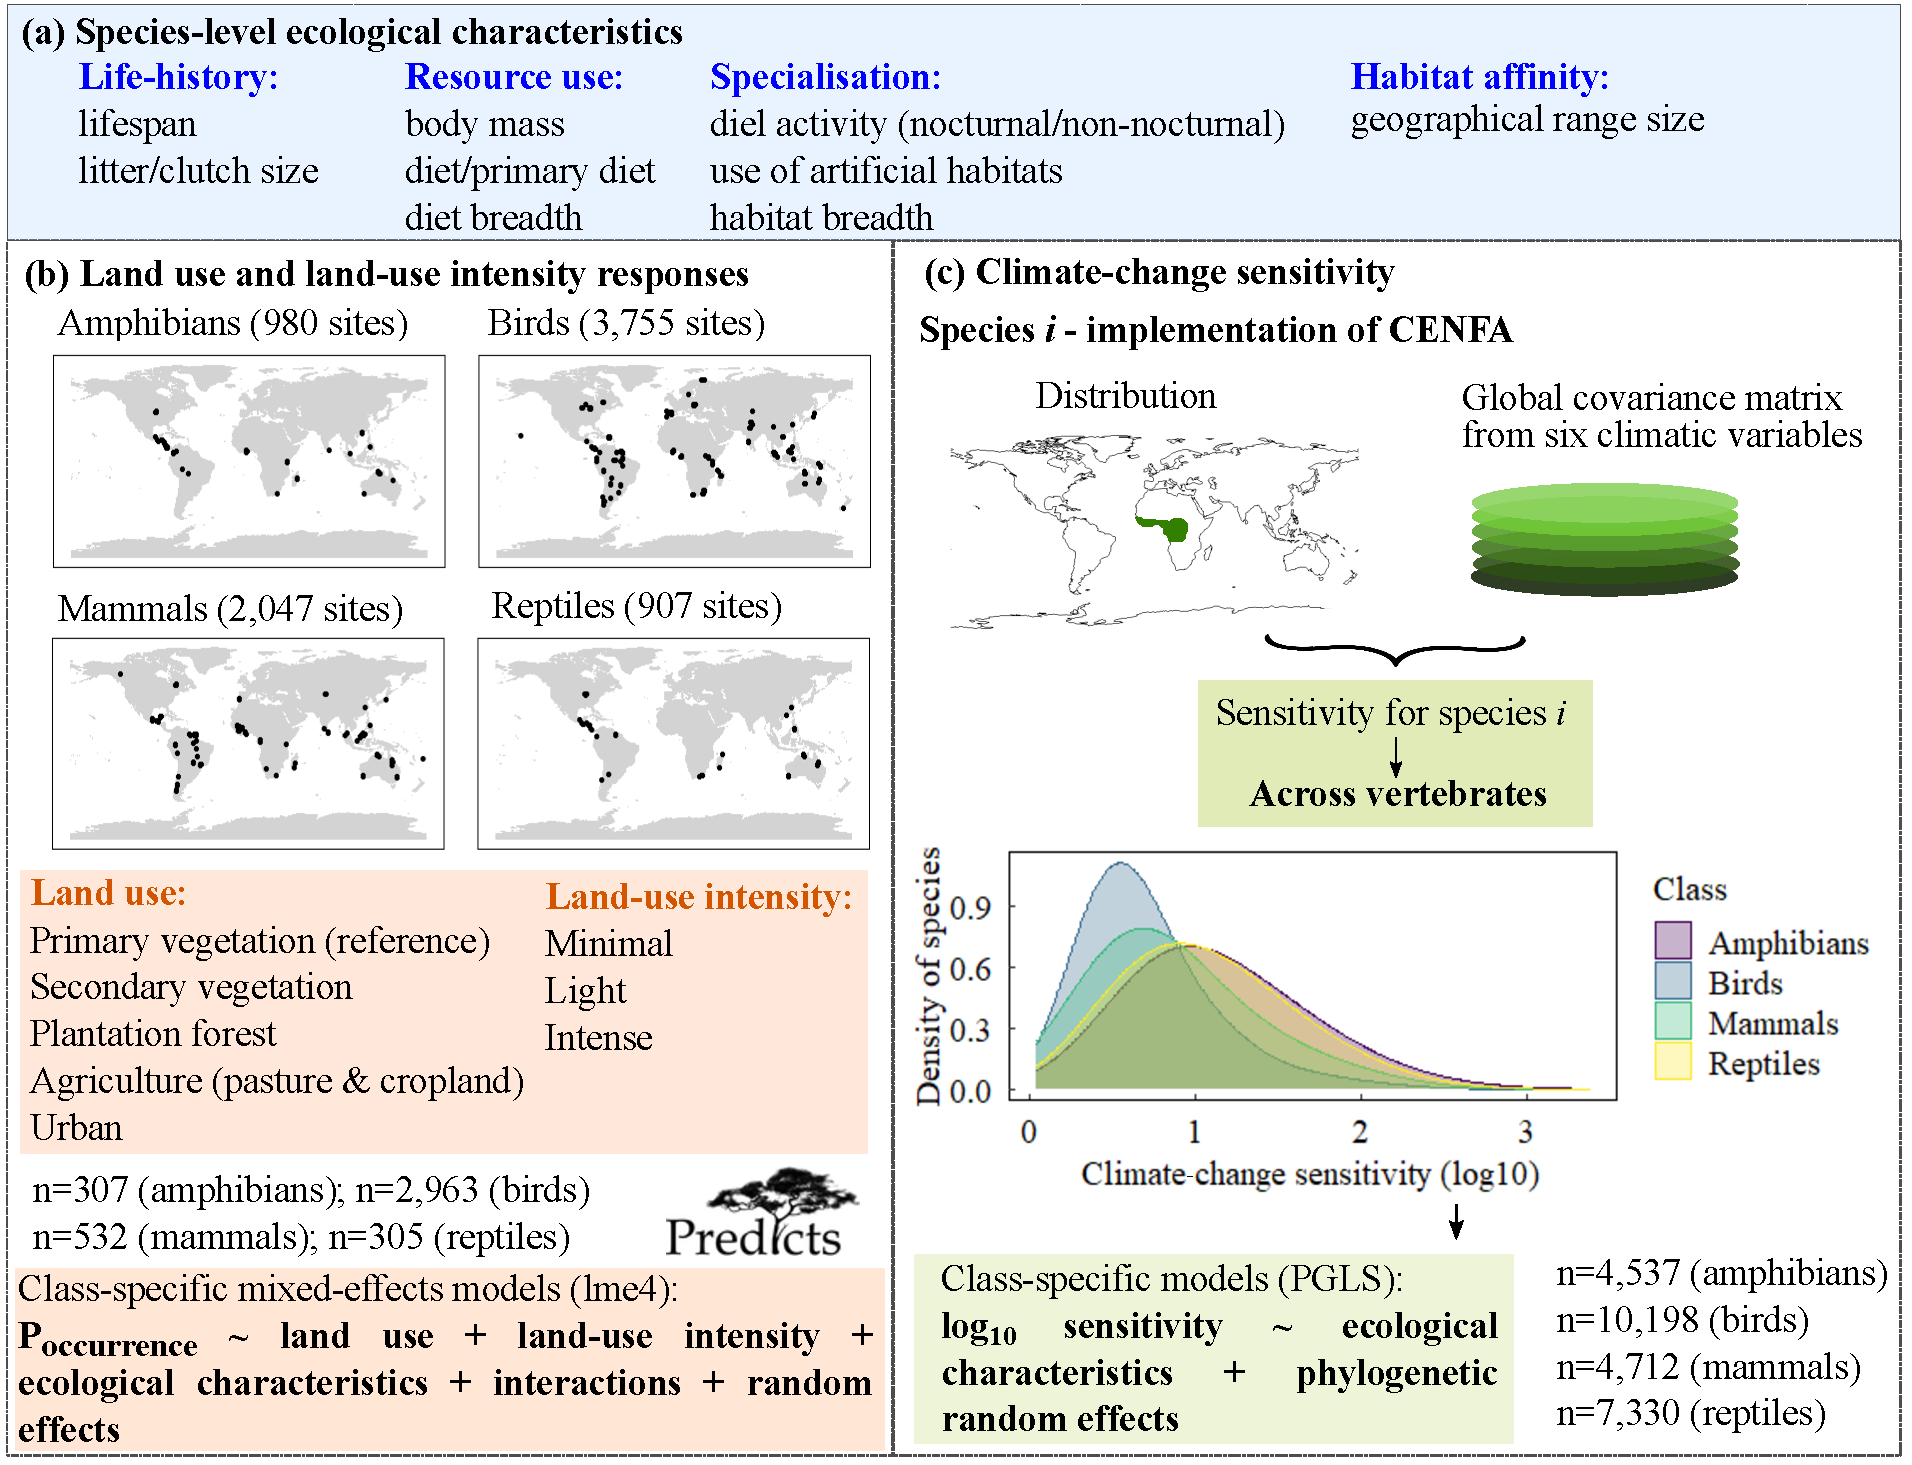
\includegraphics[scale=0.55]{figures/Chapter4/Figure1}
\caption[Framework of the study]{\textbf{Framework of the study.} \textbf{(a)} I collected ecological trait data and geographical range areas across terrestrial vertebrates (termed `ecological characteristics'). I then used two independent approaches to assess the influence of these characteristics on species' responses to land use and on species' climate-change sensitivity. \textbf{(b)} To assess the influence of traits on responses to land use and land-use intensity in each vertebrate class, I combined the ecological characteristics with the PREDICTS database. \textbf{(c)} To estimate species' sensitivity to climate change, I used the CENFA framework \citep{Rinnan2019}, which relies on the combination of species’ distributions with climatic variables to estimate sensitivity from properties of the species’ climatic niche space. I then built class-specific models to assess whether the ecological characteristics were associated with  species' sensitivity to climate change.}
\label{chap4_fig1}
\end{figure}

\clearpage

\section{Methods}

\subsection{Ecological characteristics (Figure \ref{chap4_fig1}a)}

\subsubsection{Traits}

I obtained the six following traits from Chapter 2 (in which I presented a trait data compilation across terrestrial vertebrates): body size (body mass and/or length, depending on the class); a proxy for species lifespan (generation length for mammals and birds; age at sexual maturity for amphibians; and maximum longevity for reptiles); litter or clutch size; diel activity; habitat breadth; and use of artificial habitats. I chose these traits because 1) they were available across all vertebrate classes, at least for a subset of species, allowing for a comparative assessment; and 2) they relate to species life-history, ecology, and resource use, such that they might influence species' land-use responses and climatic niche properties (and thus expected climate-change sensitivity). I couldn't capture intraspecific variation in trait values, and instead I used single mean values for all traits.

I enhanced the trait data from Chapter 2 with species-level estimates of diet, lacking in the published database but likely important for understanding species' sensitivity to human pressures. For birds and mammals, I collected estimates of species primary diet (i.e., the diet inferred from the combination of food items totalling more than 50\% of species’ consumption), from the EltonTraits database \citep{Wilman2014}. For amphibians and reptiles, obtaining species \textit{primary} diet was not possible, as there were no data available on the relative consumption of different food items. For amphibians, the AmphiBIO database \citep{Oliveira2017} provided information on species consumption of different food items (just in terms of presence/absence in the diet, but without estimation of their percent use), so I inferred diet on the basis of these reported food items (however the coverage was low, with more than 75\% of the species missing diet information; Appendix 3, Figure \ref{SI_4_fig1}). For reptiles, there was no available data collection describing diet. For both reptiles and amphibians, I supplemented the existing datasets with data on species consumption from published sources (recording the presence/absence of different food items in species consumption; data compiled by Rhiannon Osborne-Tonner), for an additional 108 amphibians and for 239 reptiles (see Appendix 3, S4.1: `Compiling diet information'). 

I standardised the diet data across the vertebrate classes, by grouping species in five different diet categories: vertebrate eaters; invertebrate eaters; plant/seed eaters; fruit/nectar eaters; and omnivores  (for mammals and birds, species were classified as omnivores when all food items had a percent use $\leq$50\%; and for amphibians and reptiles, when species where known to consume both plant and animal matter, or both invertebrates and vertebrates). I also calculated species diet breadth -- the total number of recorded food items (in terms of presence/absence) known to be consumed by a species. More information on the compilation of dietary information can be found in Appendix 3, S4.1: `Compiling diet information'. 

\subsubsection{Geographical range area}
I used extent-of-occurrence maps from BirdLife International for birds (\url{http://datazone.birdlife.org/species/requestdis}), from the IUCN Red List for mammals and amphibians \citep{IUCN2020}, and from \citet{Roll2017} for reptiles (all downloaded in April 2020). I excluded areas occupied during non-breeding seasons and areas falling outside species known elevational limits (following Chapter 2). The range maps were then converted to the raster format (`raster' package, version 3.5.15 \citet{rasterpackage}), and I estimated species geographical range areas using a resolution of 1 km$^2$ with Behrmann's equal-area projection.  Although range area cannot be considered a trait (which is a property measurable at the level of individual organisms), I included range area in the analyses because past work has shown that range area is an important correlate of species' responses to land-use \citep{Newbold2018a} and climate change \citep{Thuiller2005}. In addition, range area may correlate with other aspects of species' ecology that I could not include directly in the analysis because of limited data availability, such as dispersal ability \citep{Capurucho2020}.

\subsubsection{Phylogenies}
I used information on species' phylogenetic position in the imputations of missing trait values (see next section), and also to control for phylogenetic relationships in the models investigating the association between species' ecological characteristics and species' estimated climate-change sensitivity. Class-specific phylogenetic trees were downloaded April 2020 from \url{https://zenodo.org/record/3690867#.Xyc5wyhKhPZ} for mammals (Phylacine 1.2; \citet{Faurby2018, Faurby2020}); and from \url{https://data.vertlife.org/} for amphibians \citep{Jetz2018}, birds \citep{Jetz2012} and squamates \citep{Tonini2016}. For each class, I used a consensus tree obtained with the TreeAnnotator programme of the BEAST software (Bouckaert et al. 2014), from an available distribution of 1000 trees. 

\subsection{Imputations of missing trait values}
For some of the traits and classes, there was a substantial proportion of missing trait values (Figure \ref{SI_4_fig1}). To fill these gaps, I imputed missing trait values using random forests, as implemented with the `missforest’ function of the `missForest’ package in R (version 1.4, \citet{Stekhoven2012, Stekhoven2016}). `missforest' is one of the best methods for missing-value imputations when working with continuous and categorical variables, and when including species phylogenetic position as a predictor \citep{Penone2014, Debastiani2021}. After showing that several traits were strongly phylogenetically conserved (Table \ref{SI_4_Table1}), I included ten phylogenetic eigenvectors in the imputations \citep{Penone2014}, as well as taxonomic orders as a categorical variable (included to account for the taxonomic positions of species that were not represented in the phylogenies). Full details are given in Appendix 3 (S4.2: `Imputing missing trait values'). After imputation, continuous traits were log$_{10}$-transformed to improve normality (except for habitat and diet breadth, which I square-root transformed; this transformation was more appropriate here because the distributions of habitat breadth and diet breadth tended to be less right-skewed than that of the other traits, and the range of values was smaller).

\subsection{Characterizing the influence of traits on species' land-use responses (Figure \ref{chap4_fig1}b)}

\subsubsection{Vertebrate assemblage composition}

To compare vertebrate assemblages in different land-use types, I used the PREDICTS database \citep{Hudson2014, Hudson2017}. PREDICTS is a collection of independent studies that have sampled biodiversity in sites of varying land use and land-use intensity. Samples are mostly of species abundance, sometimes species occurrence, and rarely just overall species richness. It is one of the most comprehensive such databases to date, with 4,107 vertebrate species sampled across 7,689 sites considered in this work (Figure \ref{chap4_fig1}b). In PREDICTS, sites are assigned to one of the following land-use categories: primary vegetation (native vegetation); secondary vegetation, plantation forest, pasture, cropland, and urban (disturbed land uses; see Table \ref{SI_4_Table2} and \citet{Hudson2014, Hudson2017} for more details). Each site is also characterised in terms of land-use intensity based on land-use-specific criteria (such as mechanisation degree, crop diversity and agricultural inputs for cropland; \citet{Hudson2014}). Land-use intensity is divided into three categories to reflect the degree of human transformation and impacts on the land: minimal, light or intense. Here, I considered minimally-used primary vegetation to be the least-disturbed reference land use against which I compare all other land-use types. I grouped pasture and cropland together into a category I termed `agricultural'. As the design of the PREDICTS database is not balanced, sample sizes varied among classes and land-use types (Figure \ref{SI_4_Figure4}).

\subsubsection{Full models (all-predictor models)}

Within each vertebrate class, I investigated whether interactions among the ecological characteristics, land use and land-use intensity explained species occurrence probability. I fitted four binomial mixed-effects models (one for each class), using the `lme4' package (version 1.1-23; \citet{Bates2015}), with random effects accounting for study, site and species identity to account for the nested design of the database, taxonomic non-independence, and repeated observations among species. I did not consider interactions among the ecological characteristics, but I included interactions between land use and ecological characteristics, and between land-use intensity and ecological characteristics. Before fitting the models, I checked the degree of multicollinearity among explanatory variables using generalised variance inflation factors (GVIF; \citet{Fox1992}), with a threshold of 5 for the detection of multicollinearity (Tables \ref{SI_4_Table3}-\ref{SI_4_Table8}). For amphibians and reptiles, including both diet and diet breadth was problematic, so I excluded diet from the set of predictors for these classes on the basis of the GVIF scores. Models investigating the effects of diet were built separately (see next section, `Partial models').

I did not use phylogenetic random effects directly in the models because of the computational load required by such models when working with several hundred or thousands of species. However, I checked the phylogenetic signal in the models' residuals using Pagel’s $\lambda$ \citep{Pagel1999}. Thus, in each class, the model fitted was:\\
\\
$\text{P\textsubscript{occurrence}}\sim \text{land use} + \text{land-use intensity} + \text{species-level ecological characteristics} + \\
\text{land use}:\text{species-level ecological characteristics} + \\
\text{land-use intensity}:\text{species-level ecological characteristics} + \\
(1|\text{study identity}) + (1|\text{site identity}) + (1|\text{species identity})$.\\

To verify that the models' estimates were robust to any violation of distributional assumptions, I fitted the models again using a Bayesian framework (using the `MCMCglmm' package version 2.32, \citet{mcmcglmm}).

\subsubsection{Partial models (single-predictor models)}
In addition to the full models, I fitted partial models for each class. These were fitted to visualise occurrence patterns for each trait independently of other traits. The structure of the models was similar to that of the full models, except that I included a single species-level characteristic at a time in each model. 

\subsubsection{Effects of categorical ecological characteristics on species' occurrence probability (Figure \ref{chap4_fig2}a)}
The influence of categorical traits on species' responses to land use and land-use intensity can be visualised in two ways: either by comparing occurrence probability in different land-use types relative to species with similar traits (I term such effects `among land-use type effects', Figure \ref{chap4_fig2}a); or by comparing occurrence probability in a given land-use type relative to species with different traits (I term such effects `within land-use type effects', Figure \ref{chap4_fig2}a). 

\begin{itemize}
\item
Within land-use type effects (Figure \ref{chap4_fig2}a): from the full, all-predictor models fitted for each class, I focused on the interactive effects between land use and ecological characteristics (and between land-use intensity and ecological characteristics). These interactions indicated whether, in a given land-use type, there were any significant differences in occurrence probability between species with different traits. In other words, I looked at whether any trait level lowered or increased occurrence probability in each land-use type, compared to a reference trait level. I used this approach for all the categorical predictors, except diet (interpreting within land-use type effects for primary diet being complicated by the fact that there were more than two levels for this trait).  
\item
Among land-use type effects (Figure \ref{chap4_fig2}a): from a partial model, I predicted occurrence probability in the different land uses for all different levels of the trait. The partial models allowed to visualise occurrence patterns across land-use types for single explanatory variables, without having to account for the values of other variables. I used this approach to evaluate the influence of diet on species' land-use responses.
\end{itemize}


\subsubsection{Effects of continuous ecological characteristics on species’ occurrence probability (Figure \ref{chap4_fig2}b)}
For a given continuous ecological characteristic, any effect of land use or land-use intensity can be assessed through changes in the slope of the relationship between the ecological characteristic and occurrence probability (Figure \ref{chap4_fig2}b). When an ecological characteristic negatively impacts occurrence probability in a disturbed land use, I expect the slope of the relationship to be more negative than the slope for the reference land use (minimally-used primary vegetation). Focussing on slopes does not allow to infer absolute changes in occurrence probability across land-use types (e.g., a positive slope in a disturbed land use does not mean that there are absolute increases in occurrence probability in that land use, but only that higher values of the ecological characteristic are associated with relatively higher occurrence probability in that land-use type). This is because I do not assess changes in the mean occurrence probability here (which would require to consider the intercept of the relationship between the ecological characteristic and occurrence probability in different land-use types). Thus, I only capture `within land-use type' effects for continuous predictors.

\vspace{0.5cm}
%% Figure 2 = assessing effects 
\begin{figure}[h!]
\centering
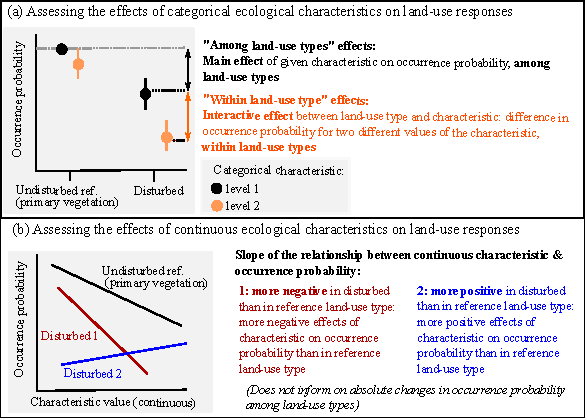
\includegraphics[scale=1.6]{figures/Chapter4/Figure2}
\caption[Assessing the effects of ecological characteristics on species' land-use responses: methodology for (a) categorical characteristics and (b) continuous characteristics.]{\textbf{Assessing the effects of ecological characteristics on species' land-use responses: methodology for (a) categorical characteristics and (b) continuous characteristics.} \textbf{(a)} For all categorical characteristics, except diet, I look at `within land-use type' effects, asking whether there are significant differences in occurrence probability among species with different ecological characteristics in a given land-use type. For diet, I look at `among land-use type' effects, comparing species occurrence probability in disturbed land uses versus that in primary vegetation  (I chose this approach here because visualising `within land-use type' effects for diet is complicated by the fact that there were more than two levels for this categorical trait). \textbf{(b)} For continuous characteristics, I focus on the relationship with occurrence probability, and I investigate how the slope of this relationship is affected by land-use type, i.e. a `within land-use type' effect.}
\label{chap4_fig2}
\end{figure}

\subsubsection{Validation on complete trait data subset (no imputed trait values)}
To assess whether the results were robust to trait imputation uncertainty, I fitted the models again for the subset of species for which I had complete, non-imputed data for all ecological characteristics. The models' structure was unchanged for birds and mammals. For amphibians, I excluded both diet and litter/clutch size because of multicollinearity issues, and I also excluded lifespan proxy and body mass (as there were too many missing values in the dataset, 85\% and 59\% respectively). For reptiles, I excluded both diet and body mass because of multicollinearity issues.

\pagebreak

\subsection{Characterizing the influence of traits on species' sensitivity to climate change (Figure \ref{chap4_fig1}c)}

I estimated climate-change sensitivity across vertebrate species using the `Climate-niche Factor Analysis' (CENFA) approach developed by \citet{Rinnan2019}, implemented with the `CENFA'  R package  version 1.1.1 \citep{CENFA}. CENFA is a spatial approach for estimating species' climate-change sensitivity, exposure, and vulnerability. CENFA combines distribution data with climatic variables to estimate sensitivity and vulnerability from properties of species' climatic niches (see \citet{Rinnan2019} for details). CENFA has been used in previous studies focused on a small number of species or on a few taxonomic groups, but to my knowledge has not yet been applied across all terrestrial vertebrates.

\subsubsection{Historical climate data}
I used global climate data  from WorldClim version 2.1 \citep{Fick2017}. I downloaded 19 climatic variables at a resolution of 2.5 arcminutes ($\sim$4.6 km$^2$ at the Equator). I removed variables that were strongly collinear with any other climatic variables (using a threshold of 0.65 for Spearman correlation coefficients). I obtained six groups of intercorrelated variables (using the `removeCollinearity' function from the `virtualspecies' R package version 1.5.1 \citep{virtualspecies}; Figure \ref{SI_4_Figure5}), and randomly selected one climatic variable in each group. The final set comprised six climatic variables: annual mean temperature (bio1), mean diurnal temperature range (bio2), maximum temperature of the warmest month (bio5), annual precipitation (bio12), precipitation seasonality (bio15), and precipitation of the coldest quarter (bio19).

\subsubsection{Estimating climate-change sensitivity from CENFA}
All climatic variables and distribution files were re-projected to a resolution of 5 km$^2$ in the Behrmann equal-area projection. I picked this resolution because the coarser the resolution, the more climate-change sensitivity tended to be underestimated for narrowly distributed species (Figures \ref{SI_4_Figure6} \& \ref{SI_4_Figure7}). However, finer resolutions demand a large amount of memory space when working at global scales across all terrestrial vertebrates. I found the 5-km$^2$ resolution to be an acceptable trade-off between computational load and accuracy of the sensitivity estimations. However, when working at 5-km$^2$ resolution, there were still some narrowly distributed species for which sensitivity was likely underestimated (Figure \ref{SI_4_Figure7}). Thus, I chose to exclude species with a range area $\leq$100 km$^2$ from further analyses (i.e., excluding narrow-ranging species whose distributions could intersect up to 4 grid cells). In doing so, the sample size was reduced by 660 species for amphibians, by 142 species for birds, by 129 species for mammals, and by 615 species for reptiles (the final sample sizes were: n=4,537 for amphibians; n=10,198 for birds; n=4,721 for mammals; n=7,330 for reptiles). My results were overall robust to the exclusion of these species (see Results section). 

I then combined the climate data with the species' distributions to estimate sensitivity to climate change, applying the CENFA framework across terrestrial vertebrates (Figure \ref{chap4_fig1}c). Further details of the implementation of the CENFA framework are given in Appendix 3 (S4.5: `Implementing Climate-niche Factor Analysis across terrestrial vertebrates').


\subsubsection{Climate-change sensitivity models}
I used phylogenetic least-square (PGLS) regressions, implemented in the `caper' R package version 1.0.1 \citep{caper}, to assess the effects of ecological characteristics on species' estimated sensitivity to climate change, while controlling for phylogenetic relationships among species. I combined the ecological characteristics and the phylogenies using the `comparative.data' function from the `caper' package, and then built class-specific models to explain climate-change sensitivity with the ecological characteristics (Figure \ref{chap4_fig1}c). Before fitting the models, I checked for multicollinearity among the predictors using GVIF scores. Across all classes, the models included all the main effects of the ecological characteristics, except for amphibians, for which I dropped diet breadth (which was strongly collinear with diet; Tables \ref{SI_4_Table9}-\ref{SI_4_Table13}). For the continuous predictors, I fitted third-order polynomials to allow for non-linearity of the responses (I included third order polynomials for the climate-change sensitivity models but not for the land-use models because the PGLS model had a simpler structure than the land-use models, were less computationally intensive, and also because the number of estimated parameters was already high for the land-use models without allowing for third-order polynomials). As such, the general form of the PGLS models was: 
\\
$\log_{10}\text{(climate-change sensitivity)}  \sim  \text{poly(log\textsubscript{10}(continuous ecological characteristics),3)} + \\
\text{categorical ecological characteristics} + \\
\text{phylogenetic random effects}$.


\subsubsection{Models' robustness}

\begin{itemize}

% exclusion of species with RS>100km2
\item To check whether the results were robust to the exclusion of species whose range area was $\leq$100 km$^2$, I repeated the models on all species (including those with range area $\leq$100 km$^2$: n=5,208 for amphibians; n=10,340 for birds; n=4,844 for mammals; n=7,951 for reptiles). 

% Minor corrections  - breeding range vs non-breeding range
\item For birds and mammals, I further checked whether the results were robust to the exclusion of migratory species, for which breeding and non-breeding ranges could differ, possibly impacting the definition of species climatic niche spaces. I identified migratory mammals using the dataset from \citet{Gnanadesikan2017}, and migratory birds from BirdLife international (check how to cite / acknowledge). 

% Minor corrections - different resolutions
\item I further checked whether the results were sensitive to different resolutions. Resolution can have an impact on climate-change sensitivity (e.g., coarser resolutions tend to underestimate climate-change sensitivity of narrow-ranging species Figure S\ref{}). 

% robustness to imputations
\item Finally, to assess the degree to which the results were robust to trait imputation uncertainty, I fitted the models again for the subset of species for which I had empirical (i.e., non-imputed) trait estimates. Diet was excluded for amphibians and reptiles on the basis of high collinearity (GVIF$>$5). I fitted first-order polynomials here because of the substantially reduced sample size compared to the main models.

\end{itemize}




\section{Results}

\subsection{Land-use responses}

\subsubsection{`Within land-use type' effects (Table \ref{chap4_table1}a)}
Land-use, land-use intensity, species' ecological characteristics and their interactions had significant effects on species occurrence probability. Significant interactive effects between land use and ecological characteristics (and between land-use intensity and ecological characteristics) reflected differences in the ability of species with different ecological characteristics to cope within the disturbed land-use types (Table \ref{chap4_table1}a). Across all classes, species with narrower geographical range areas, smaller habitat breadth and inability to exploit artificial habitats showed greater decreases in occurrence probability within disturbed land uses, than species with larger range areas, larger habitat breadth and ability to exploit artificial habitats (the only exceptions were opposite effects found for mammals and reptiles for habitat breadth in two of the land-use types). The effects of the other ecological characteristics differed in direction depending on class and land use, impeding any generalisation (Table \ref{chap4_table1}a). For instance, I found that being smaller and longer-lived was associated with decreases in occurrence probability for birds found in agricultural areas, but with increases in occurrence probability for urban birds; and that  longer-lived species tended to be more negatively affected for mammals and reptiles, whereas I found evidence of opposite trends for amphibians.

I would like to highlight that the `within land-use type' effects summarised in Table \ref{chap4_table1}a do not necessarily reflect occurrence patterns among land-use types. For example, in all classes, `among land-use type' effects derived from partial models showed that occurrence probability in disturbed land uses was strongly negatively affected for natural habitat specialists, compared with primary vegetation levels (Figure \ref{SI_4_Figure10}). On the other hand, in most classes and disturbed land uses, artificial habitat users either increased or showed no significant difference in occurrence probability. One exception was for reptiles, where the effect of habitat specialisation was mostly non-significant within land-use types (Table \ref{chap4_table1}a), with both natural habitat specialists and artificial habitat users showing important declines in some disturbed land uses (e.g., intensely-used agricultural areas, Figure \ref{SI_4_Figure10}d). Similarly, the occurrence probability of both nocturnal and non-nocturnal species was negatively impacted in disturbed land uses compared with primary vegetation (Figure \ref{SI_4_Figure11}), such that land-use responses were not distinguishable between nocturnal and non-nocturnal species for all classes and land-use types. 


%% Synthesis table 
\begin{landscape}
\begin{table}
\centering
\caption[Summary of the effects of the ecological characteristics (except for primary diet) on species' responses to disturbed land uses (`within land-use type' effects) and on species' climate-change sensitivity, for each Class of terrestrial vertebrates.]{\textbf{Summary of the effects of the ecological characteristics (except for primary diet) on (a) species' responses to disturbed land uses (`within land-use type' effects) and (b) species' climate-change sensitivity, for each class of terrestrial vertebrates.} The symbol \colorbox{Salmon}{\textcolor{BrickRed}{\textbf{--}}} indicates where a characteristic has a significant negative effect on occurrence probability within a disturbed land-use type (within any of the land-use intensities), or where the characteristic renders species significantly more sensitive to climate change. A \colorbox{YellowGreen}{\textcolor{ForestGreen}{\textbf{+}}} indicates a significantly  positive effect of a characteristic on occurrence probability in a land-use type (within any of the land-use intensities), or significantly lower sensitivity to climate change. For the land-use effects, I report `within land-use type' effects here, that is, within a disturbed land use whether there were significant differences in occurrence probability among species with different trait values (see Figure \ref{chap4_fig2}). These effects were derived from the interactive terms of the full, all-predictor models.}
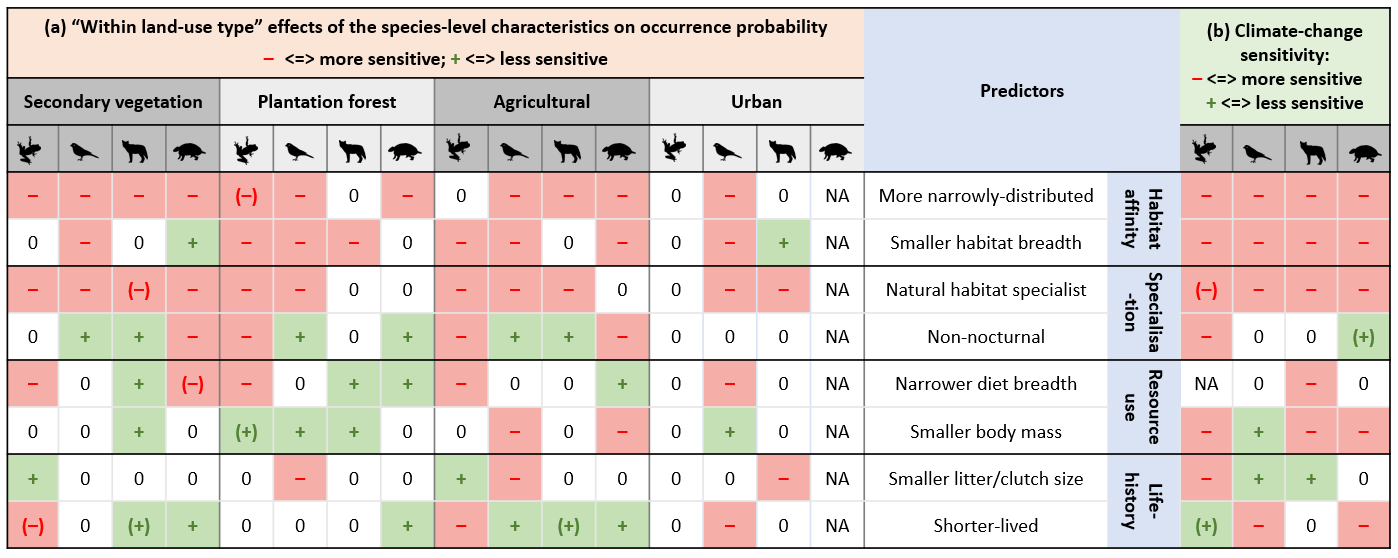
\includegraphics[scale=0.8]{figures/Chapter4/Synthesis_table}
\label{chap4_table1}
\end{table}
\end{landscape}

\subsubsection{Effects of diet on species' occurrence probability (Figure \ref{chap4_fig3})}
In all classes, diet had significant effects on occurrence probability in disturbed land uses (Figure \ref{chap4_fig3}). Changes in occurrence probability in disturbed land uses differed among classes and dietary groups. Overall, invertebrate eaters tended to be negatively affected in disturbed land uses (e.g., -66\% average declines in occurrence probability for amphibians in intensely used agricultural areas, compared with minimally-used primary vegetation). Omnivores were both negatively and positively impacted, showing both important decreases (e.g., -81\% for reptiles in intensely used plantation forest) as well as strong increases (e.g., +43\% for lightly used urban areas in birds). Overall, fruit/nectar eaters showed important declines in occurrence probability for mammals and birds, as opposed to plants/seeds eaters, whose occurrence probability tended to be strongly positively affected for birds, and dependent on land-use intensity for mammals (with increases in minimally-used land-types, but not in more intensely-used land-types). Finally, I also detected significant changes in occurrence probability for vertebrate eaters, with some declines for mammals in agricultural areas (-75\% on average in intense uses), but also some increases (e.g., +43\% on average for birds in lightly used agricultural areas).


\subsubsection{Explanatory power for the full models \& variance explained by each characteristic (Figure \ref{chap4_fig4})}
Overall, land use, land-use intensity and the ecological characteristics explained a small amount of the total variation in species' occurrence probability (marginal R$^2$: 0.15 for amphibians; 0.054 for birds; 0.15 for mammals; 0.13 for reptiles), in part because the random effects explained a substantial proportion (conditional R$^2$: 0.59 for amphibians; 0.61 for birds; 0.72 for mammals; 0.57 for reptiles). The relative importance of traits explaining the most variation differed among classes, with interactions between land use and habitat breadth explaining the most variation in amphibians and birds, but interactions between land use and body mass explaining the most variation for mammals, and interactions between land use and lifespan explaining the most variation for reptiles (Figure \ref{chap4_fig4}a). 

Finally, the models' diagnostics showed evidence of deviations from distributional assumptions (diagnostic plots for the full models are shown in Figures \ref{SI_4_Figure12}-\ref{SI_4_Figure15}). However, when estimated from a Bayesian framework, the models’ estimates were mostly congruent (results not shown), so the frequentist approach I used with `lme4' was robust despite the deviations from distributional assumptions. The phylogenetic signals in the models' residuals were low and not significant (Pagel’s $\lambda$ $<$ 0.01 for amphibians and reptiles, p $\approx$ 1; $\lambda$  = 0.13 for mammals, p = 0.09; $\lambda$  = 0.01 for birds, p = 0.56), despite not having included phylogenetic random effects.

\pagebreak
%% Diet figure
\begin{figure}[h!]
\centering
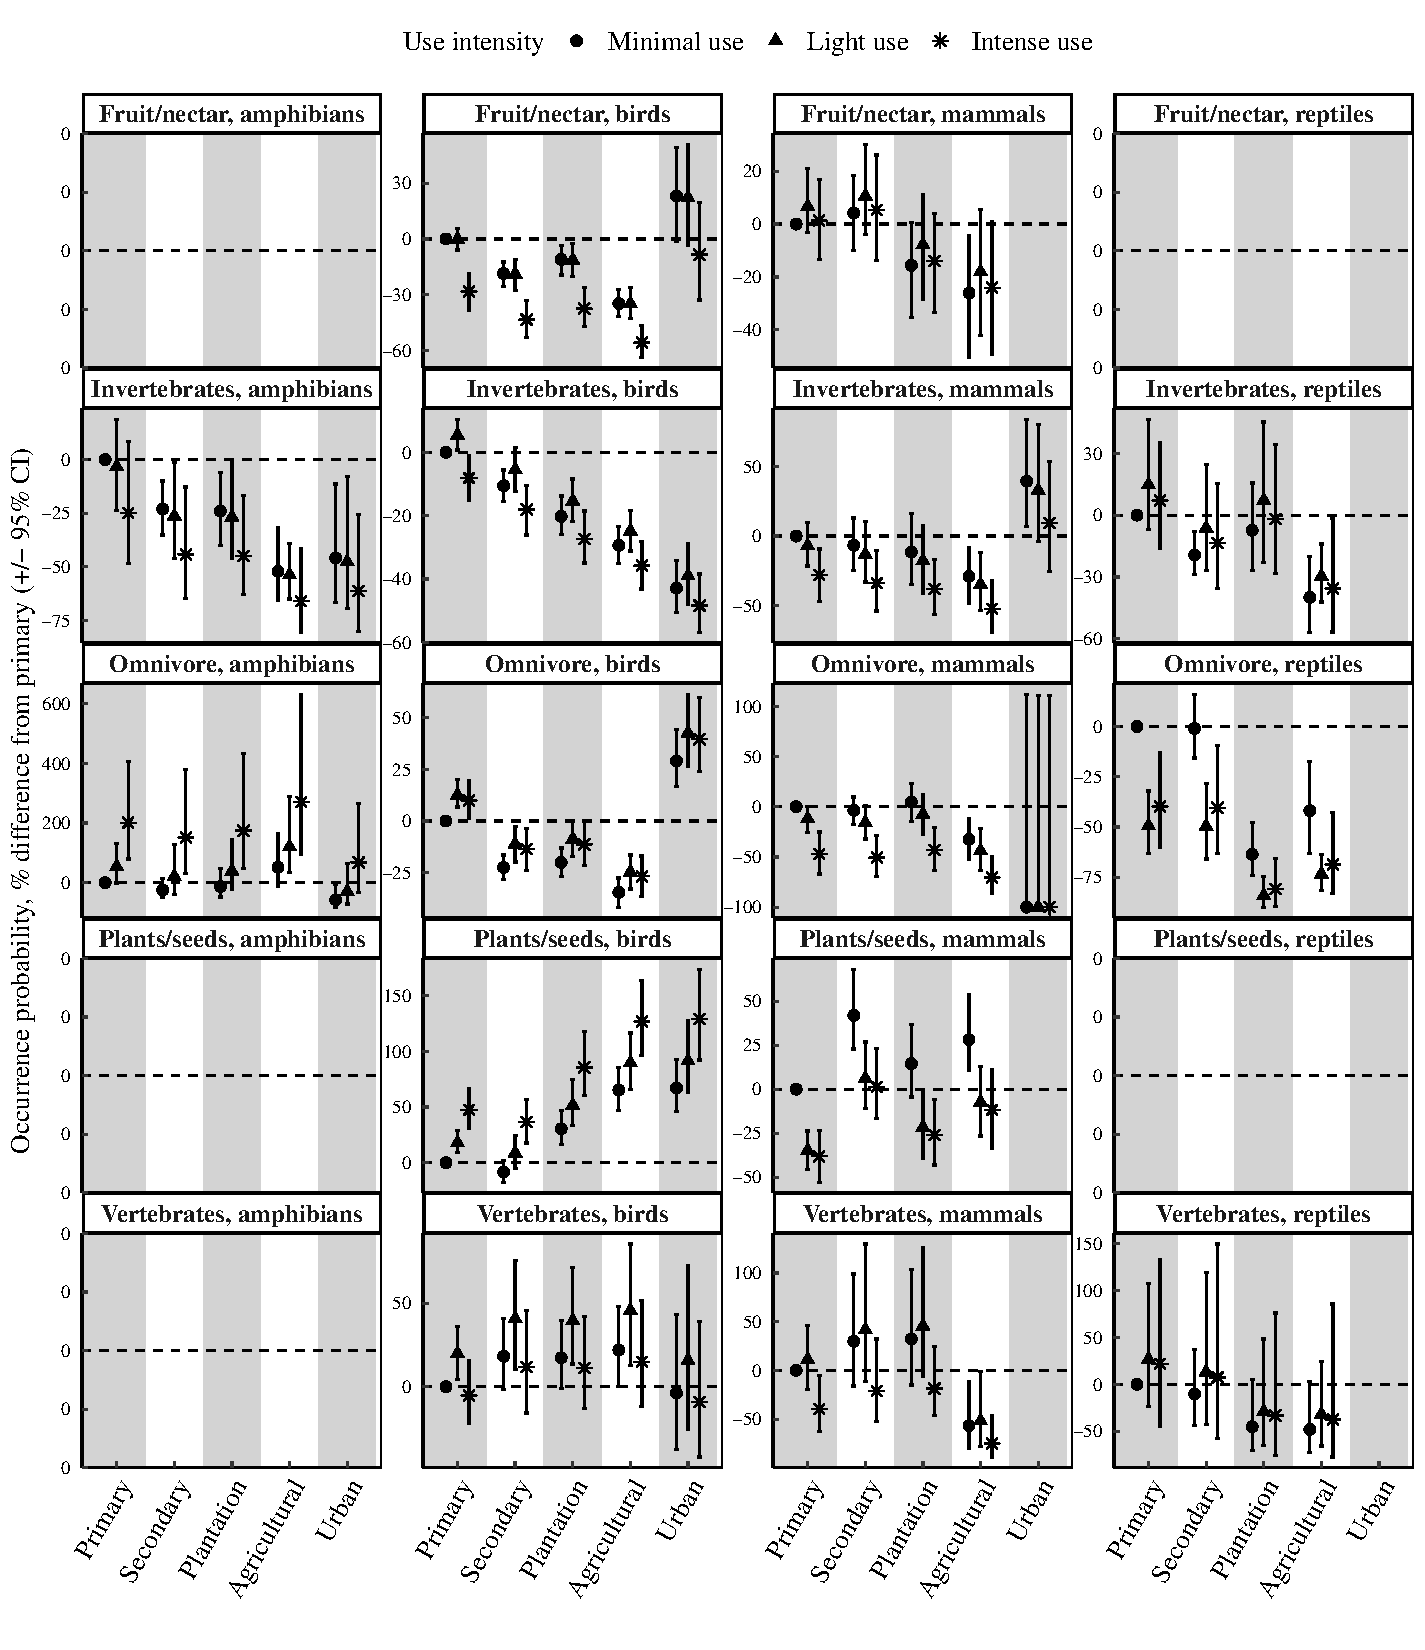
\includegraphics[scale=0.7]{figures/Chapter4/Figure3_V2}
\caption[Predicted occurrence probability as a function of land use, land-use intensity, diet and their interactions, for each class of terrestrial vertebrates.]{\textbf{Predicted occurrence probability as a function of land use, land-use intensity, diet and their interactions, for each class of terrestrial vertebrates} (mean $\pm$95\% confidence interval; the predictions are rescaled with reference to minimally-used primary vegetation). The predictions were obtained from the partial models fitted for each class, considering only diet among the ecological characteristics. Empty plots are drawn where there were no data for a diet category for a given class. Effects could not be estimated for urban reptiles, as well as for urban vertebrate, fruit/nectar and plant/seed eaters for mammals because there were no sampled species. Primary: primary vegetation; Secondary: secondary vegetation; Plantation: plantation forest; Agricultural: cropland and pasture.}
\label{chap4_fig3}
\end{figure}


\pagebreak
%% Figure Variance
\begin{figure}[h!]
\centering
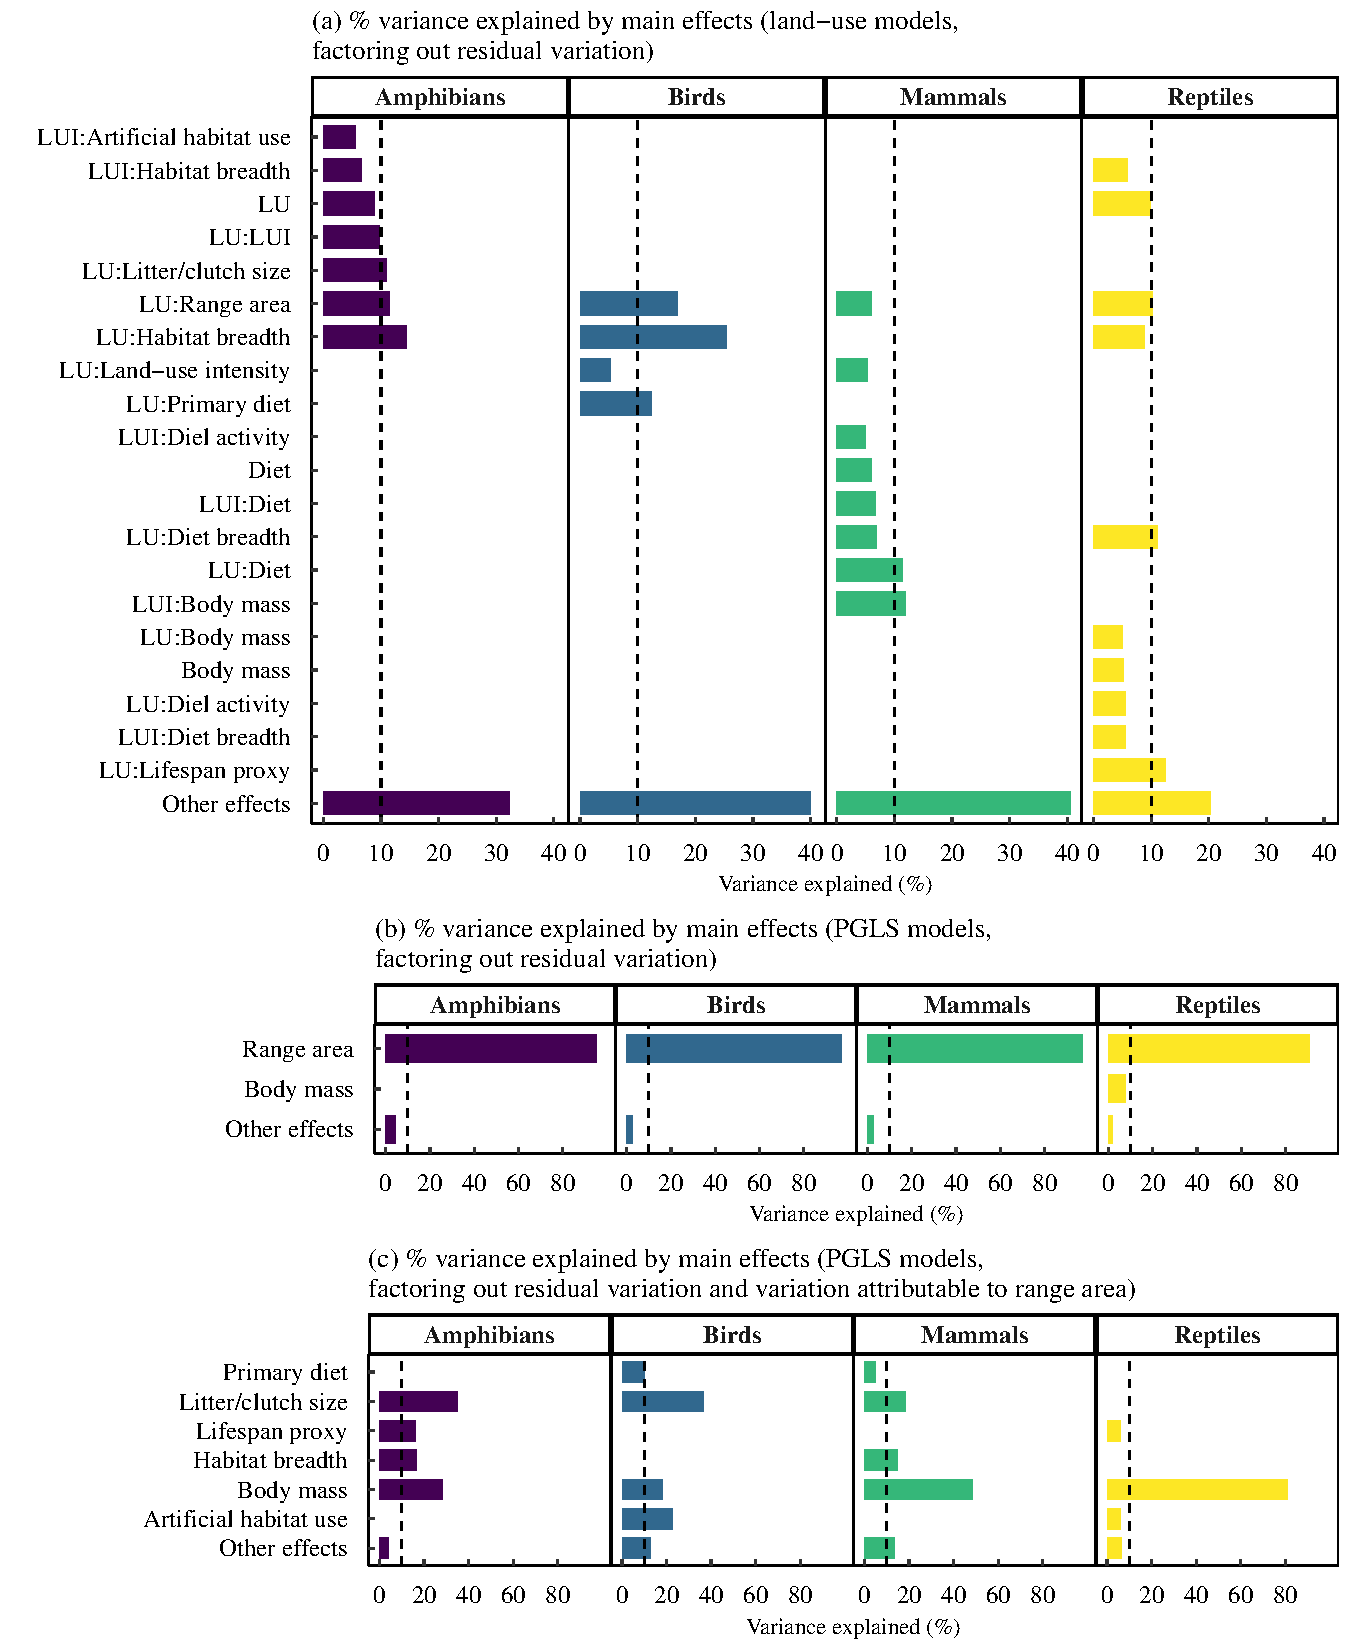
\includegraphics[scale=0.7]{figures/Chapter4/Variance_breakdown.pdf}
\caption[Proportion of the explained variance attributable to each of the main effects in the land-use and climate-change sensitivity models]{\textbf{Proportion of the explained variance attributable to each of the main effects for (a)} the mixed-effects models fitting the effects of land use, land-use intensity, and ecological characteristics on species occurrence probability (after factoring out residual variation); \textbf{(b)} for the phylogenetic least-squares regressions investigating whether the ecological characteristics explained climate-change sensitivity (after factoring out residual variation); and \textbf{(c)} for the phylogenetic least-squares regressions investigating whether the ecological characteristics explained climate-change sensitivity (after factoring out the variance explained by geographical range area and the residual variation). The dashed vertical lines mark 10\% explained variance (for visualisation purposes). I individually show all the effects that explain more than 5\% of the overall variation. Effects that individually explain less than 5\% of the overall variation are grouped together as `Other effects'. LU: land use; LUI: land-use intensity.}
\label{chap4_fig4}
\end{figure}

\clearpage
\pagebreak
\subsection{Climate-change sensitivity}
The ecological characteristics were significantly associated with climate-change sensitivity in all classes (Tables \ref{chap4_table1}b \& \ref{chap4_table2}, Figures \ref{chap4_fig5} \& \ref{chap4_fig6}); models' coefficients shown in Tables \ref{SI_4_Table14}-\ref{SI_4_Table17}). Overall, climate-change sensitivity was highest for amphibians (median log$_{10}$-sensitivity: 1.1; 95\% interpercentile range: 0.40-2.2), then reptiles (median log$_{10}$-sensitivity: 1.0; 95\% interpercentile range: 0.32-2.1), then mammals (median log$_{10}$-sensitivity: 0.76; 95\% interpercentile range: 0.22-2.0) and birds (median log$_{10}$-sensitivity: 0.62; 95\% interpercentile range: 0.21-1.77). In all classes, narrower geographical range area, smaller habitat breadth and being specialised on natural habitats were consistently associated with higher climate-change sensitivity (Table \ref{chap4_table1}b). However, other characteristics did not have consistent associations with climate-change sensitivity across classes, in different cases varying in both significance and direction. For instance, I found opposite associations between body mass and climate-change sensitivity for mammals, amphibians and reptiles on the one hand, and birds on the other hand. 


The PGLS models explained an important proportion of the overall variation in estimated climate-change sensitivity (adjusted R$^2$ = 0.64 for amphibians; 0.62 for birds; 0.63 for mammals and reptiles). Geographical range area explained the majority of this variation in climate-change sensitivity (about 60\% in all classes; Figure \ref{chap4_fig4}b), which largely reflects the design of the CENFA approach. When factoring out residual variation and variation explained by geographical range area, the relative importance of the traits as correlates of climate-change sensitivity varied among classes (Figure \ref{chap4_fig4}c), with body mass explaining the most variation for mammals and reptiles, and litter/clutch size explaining the most variation for amphibians and birds.

%% Figure climate-change sensitivity - categorical predictors
\begin{figure}[h!]
\centering
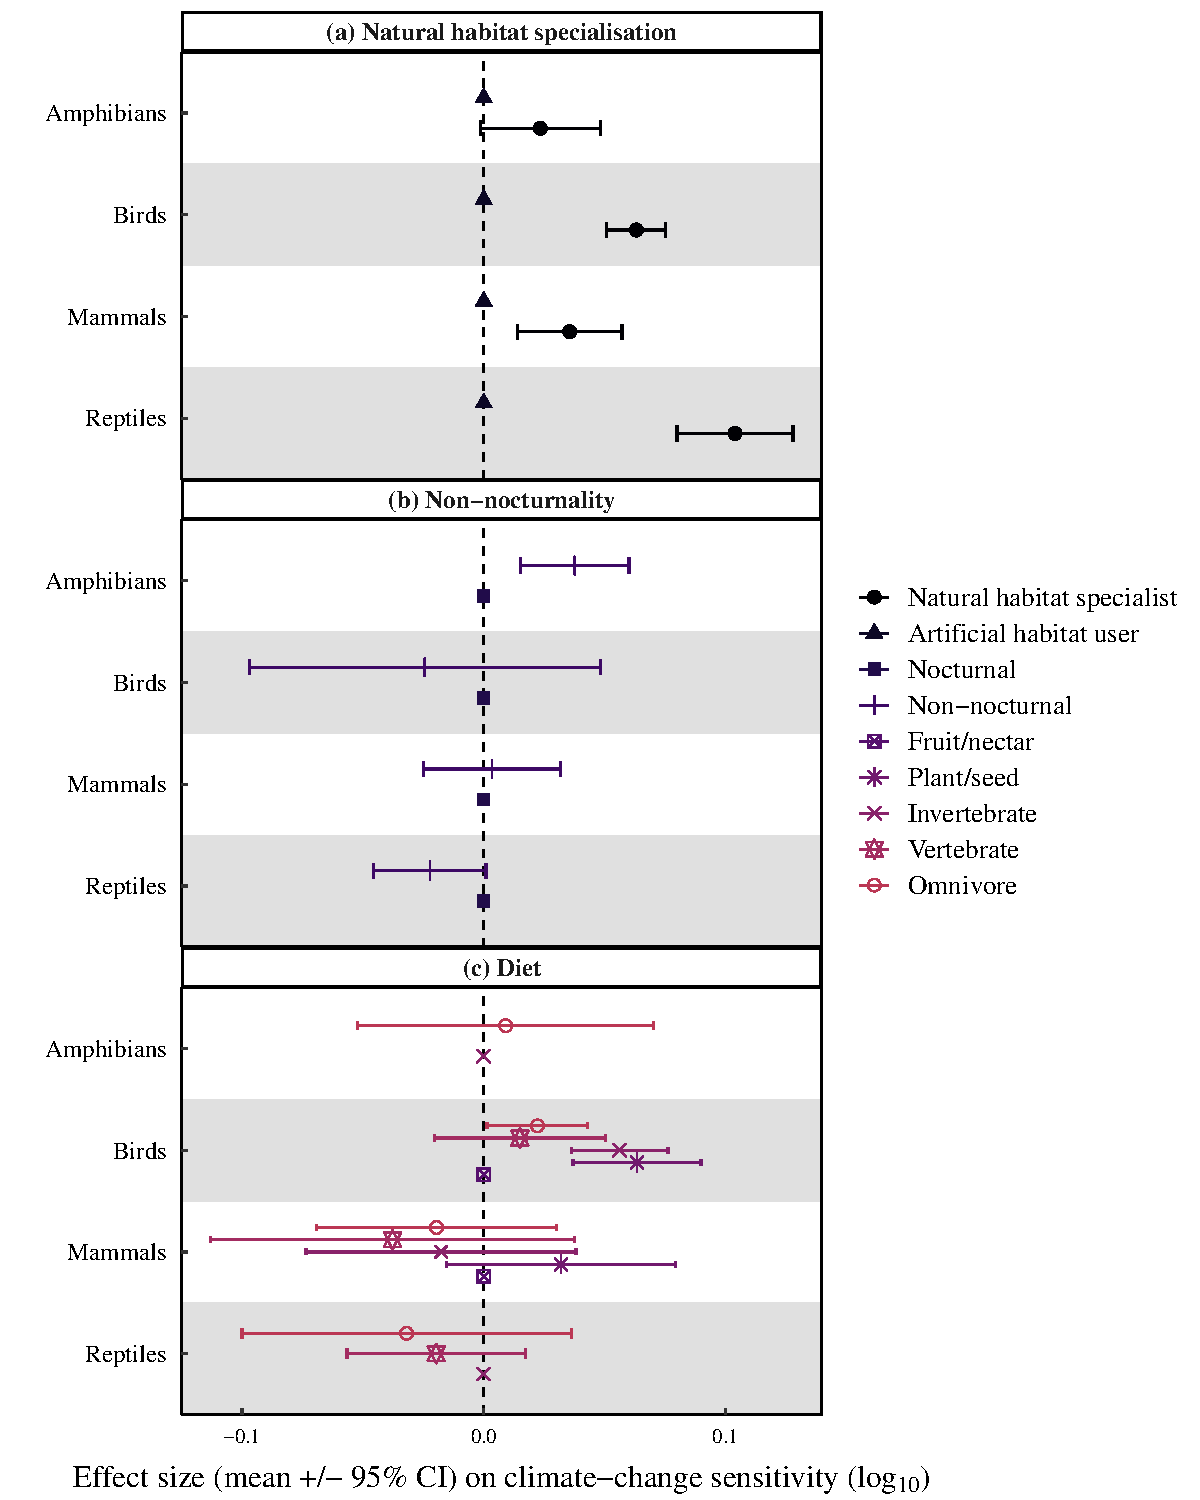
\includegraphics[scale=0.75]{figures/Chapter4/Figure5_V2}
\caption[Estimated effects of the categorical traits on climate-change sensitivity, from the PGLS models fitted in each class.]{\textbf{Estimated effects of the categorical traits on climate-change sensitivity, from the PGLS models fitted in each class (mean effect $\pm$95\% confidence interval).} For each categorical trait, I show the effect size for all levels referring to the reference level (vertical dashed line). \textbf{(a)} For artificial habitat use, the reference level is `Artificial habitat user'; \textbf{(b)} for diel activity, the reference level is `Nocturnal'; \textbf{(c)} for diet, the reference level for mammals and birds is `Fruit/nectar' eaters, but it is `Invertebrate' eaters for amphibians and reptiles. }
\label{chap4_fig5}
\end{figure}


\clearpage
%% Figure climate-change sensitivity - continuous predictors
\begin{figure}[h!]
\centering
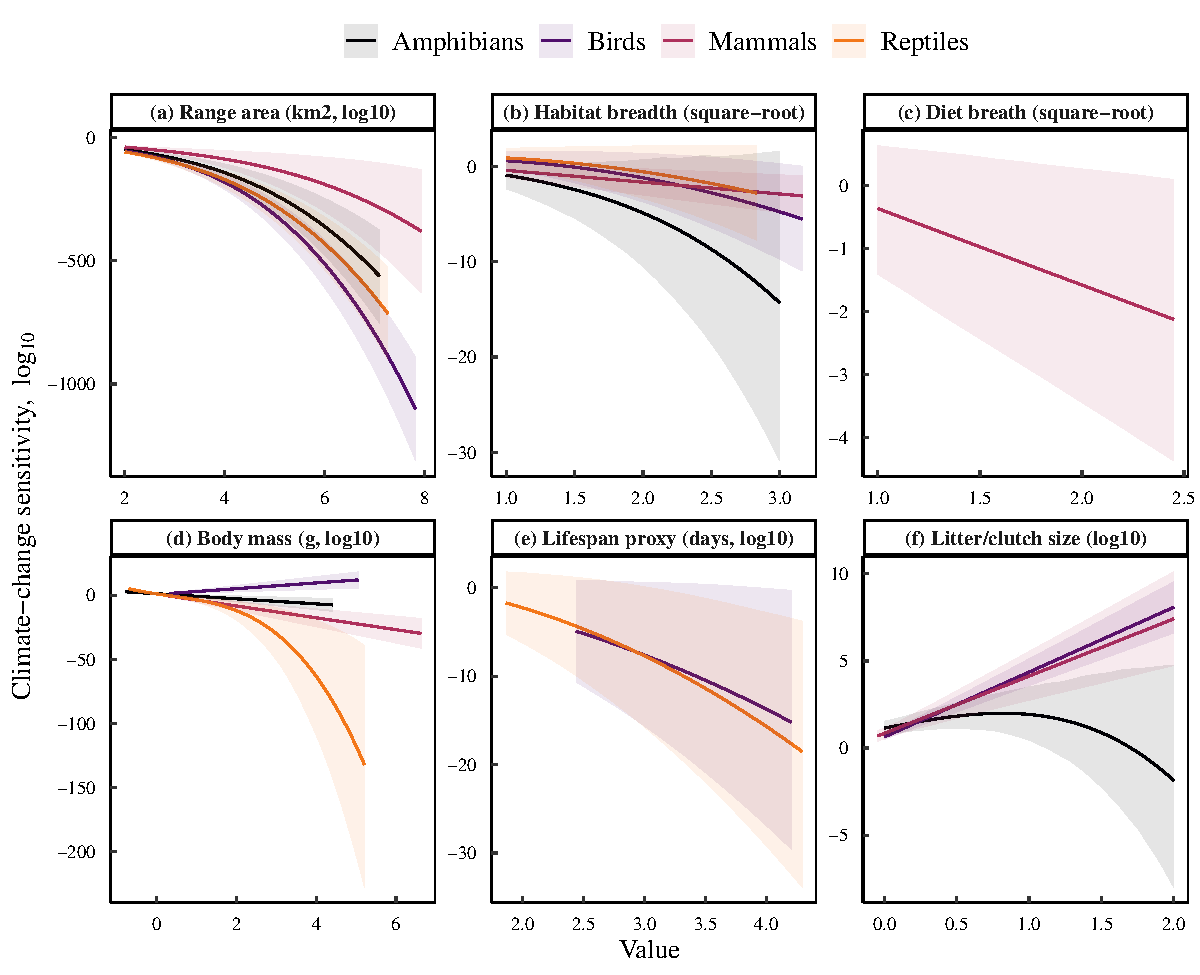
\includegraphics[scale=0.7]{figures/Chapter4/Figure6}
\caption[Effects of the continuous ecological characteristics on climate-change sensitivity, estimated from the PGLS models in each class.]{\textbf{Effects of the continuous ecological characteristics on climate-change sensitivity, estimated from the PGLS models in each class.} The lines represent the estimated relationships between climate-change sensitivity and ecological characteristics; the shaded areas are 95\% confidence intervals. I plotted the estimated relationships only when they were found to be significant.}
\label{chap4_fig6}
\end{figure}

\subsubsection{Robustness of the PGLS models}
The PGLS models were robust to distributional assumptions (Figures \ref{SI_4_Figure18}-\ref{SI_4_Figure21}). When fitting the models on all species (including those with range area $\leq$100km$^2$), I found that the relationship between climate-change sensitivity and geographical range area was reversed in all classes (with smaller-ranging species estimated to be less sensitive). This result is likely an artefact caused by the underestimation of climate-change sensitivity for the most narrow-ranging species, which would support the exclusion of such species from the analysis. Other results were generally not sensitive to the exclusion of species whose range area was $\leq$100 km$^2$ (Figure \ref{SI_4_Figure22}).

% models' summaries shown in Tables \ref{SI_4_Table17}-\ref{SI_4_Table20}.

\clearpage

%% ANOVA table for PGLS models
\begin{table}[h!]
\centering
\caption[ANOVA summaries for the PGLS models investigating the associations between the species-level ecological characteristics and species' estimated climate-change sensitivity.]{\textbf{ANOVA summaries for the PGLS models investigating the associations between the species-level ecological characteristics and species' estimated climate-change sensitivity.}}
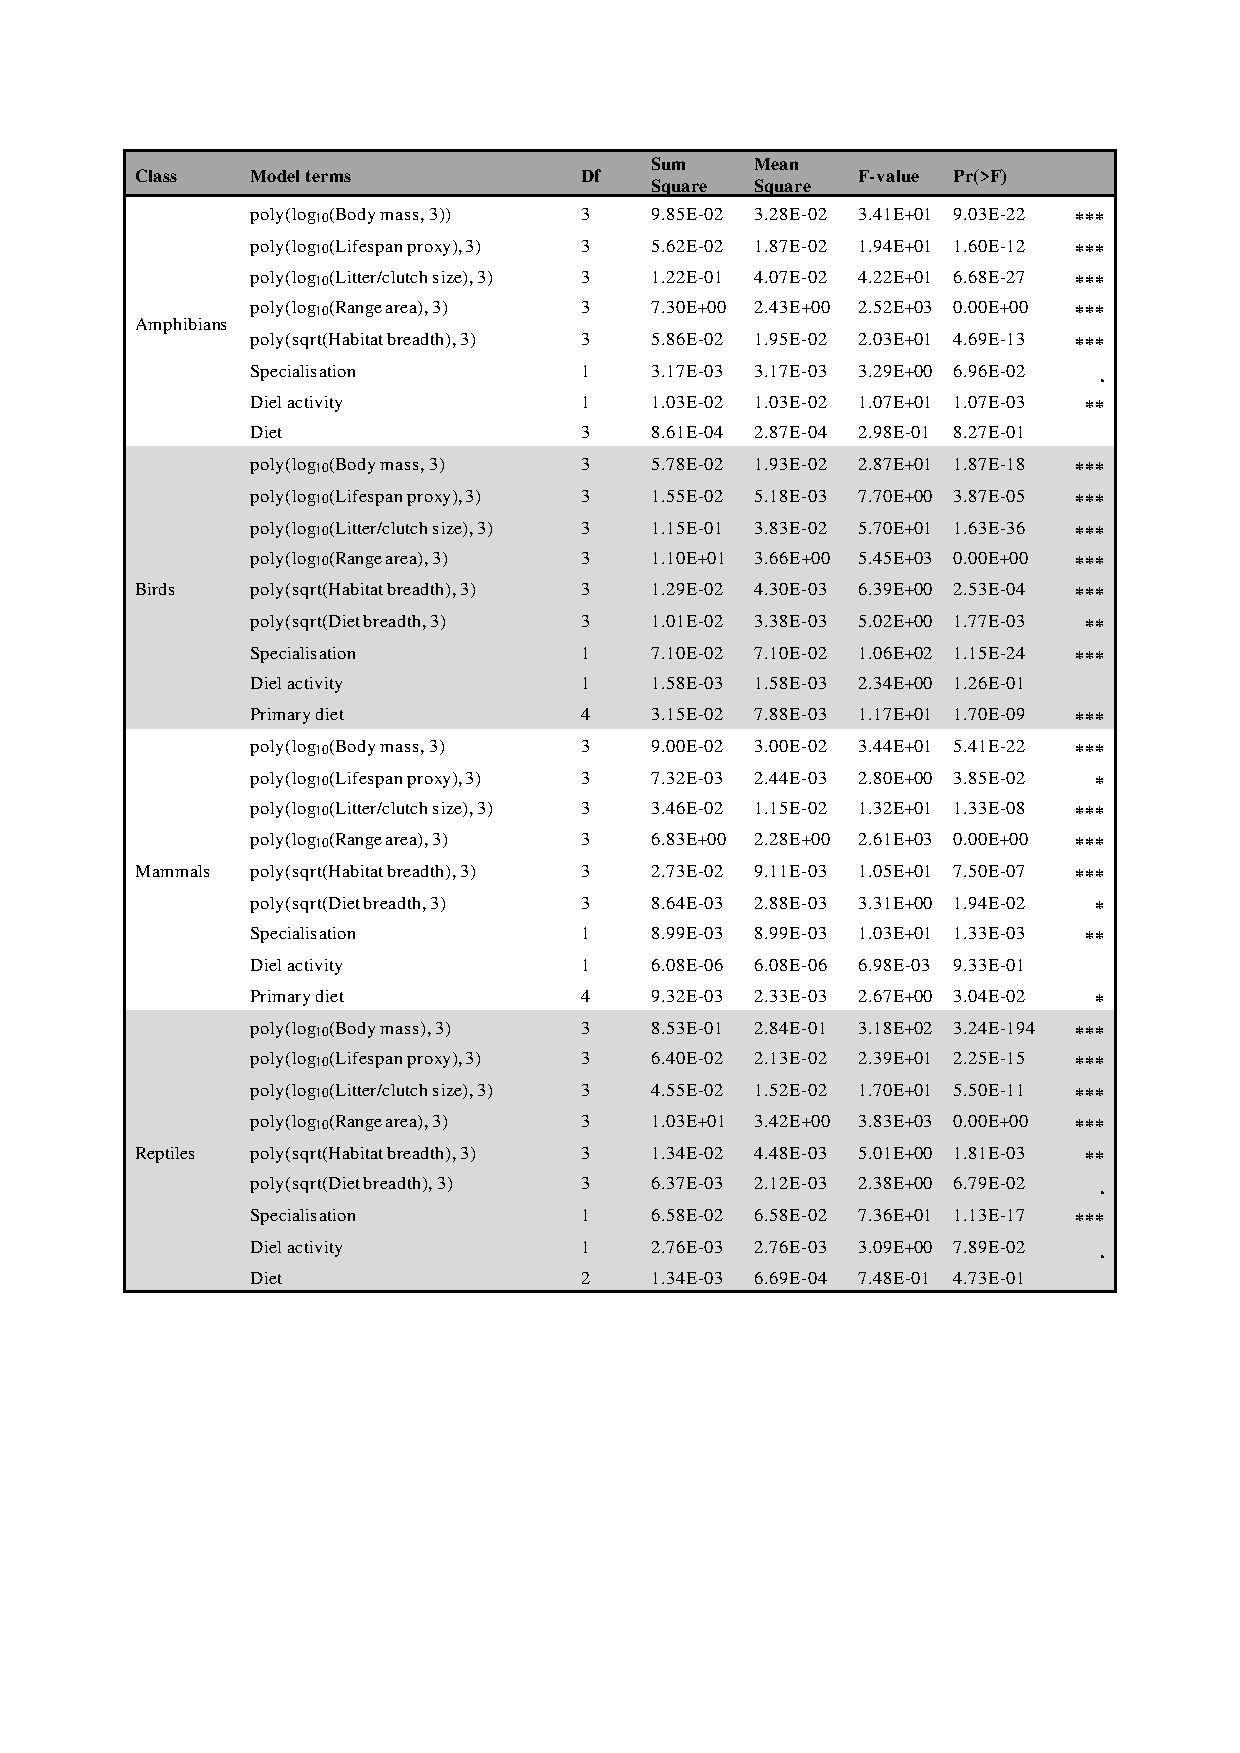
\includegraphics[scale=1, trim={2cm 5 1 2.5cm}, clip]{figures/Chapter4/Table_ANOVA_PGLS_pdf}
\label{chap4_table2}
\end{table}

\clearpage

\subsection{Validations on complete trait data}

Running the land-use and PGLS models again using data subsets for which I had empirical, non-imputed values only for the ecological characteristics showed that the conclusions of this work are likely robust to imputation uncertainty. Overall, across all classes, the associations of geographical range area, habitat breadth and use of artificial habitats with sensitivity to climate change and land-use responses were consistent with the main models (Table \ref{SI_4_Table22}, Figure \ref{SI_4_Figure23}).
%Tables \ref{SI_4_Table22}-\ref{SI_4_Table26} for models coefficients


%\clearpage

\section{Discussion}
Here, I investigated whether species' ecological characteristics were associated with species' sensitivity to two human pressures (climate change and land-use change), across terrestrial vertebrate classes. Overall, I found that geographical range area, habitat breadth and specialisation on natural habitats were consistently associated with sensitivity to both pressures across terrestrial vertebrate classes: narrower ranges, narrower habitat breadth and inability to exploit artificial habitats were associated with more negative land-use responses and with higher climate-change sensitivity. My results are in line with previous meta-analyses that have found species' extinction risks to be associated with habitat breadth and range area \citep{Chichorro2019}, range shifts under contemporary climate change to be associated with species' historical range limits and habitat breadth \citep{MacLean2017}, and with many other studies on land-use responses or extinction risks \citep{Ripple2017, Newbold2018a, Nowakowski2017, Purvis2000}. However, to the best of my knowledge, this work constitutes the first global study to compare patterns among vertebrate classes and between the two major human pressures of climate change and land use. The results of this Chapter have important implications for conservation, as they mean that land-use and climate change are non-randomly affecting all terrestrial vertebrates, with a consistently higher risk for geographically rarer species and habitat specialists. Geographical rarity has been employed by the IUCN for many years in vulnerability assessments \citep{Rodrigues2006}, and this work provides further support for its integration in large-scale assessments. My results also lend support to the idea that habitat specialisation is a likely indicator of species' sensitivity to both land-use and climate change across all vertebrates, thus indices reflecting habitat specialisation should be highly relevant to consider in large-scale vulnerability assessments, as done by \citet{Foden2013}. 

This work further highlights the class-specific associations between most traits and likely responses to human-driven environmental changes, but again highlighting a non-random reshaping of vertebrate biodiversity under global changes. In the case of land use, I find that the directionality of the responses not only often depends on taxonomic class but also on land-use type, further complicating the patterns. In line with past work highlighting the low explanatory power of traits when used to explain species' responses to human pressures \citep{Angert2011, Verberk2013, Cannistra2021}, I found that most traits explained a small proportion of the interspecific variation in land-use responses and in climate-change sensitivity. The only exception was range area, which explained a large proportion of the interspecific variation in climate-change sensitivity. Given that the estimates of climate-change sensitivity were based on properties of species' climatic niches \citep{Rinnan2019}, it was not surprising that range area explained such an important part of the interspecific variation in sensitivity, as it is likely that broader range areas are associated with broader climatic tolerances, and thus with lower estimated climate-change sensitivity on average.

Despite their generally low explanatory power, traits have been used to assess species vulnerability to human threats, in particular to climate change \citep{Foden2013, Bohm2016}. One of the conceptual appeals behind the use of traits is that if clear patterns in responses to environmental change can be identified across taxa, then it could be possible to generalize their effects in space and time \citep{Verberk2013, Hamilton2020}, which is of interest for conservation -– notably for data-deficient species and/or those lacking estimates of abundance or population sizes. This work does not provide support for the generalisation at large scales of the effects of life-history and dietary traits on sensitivity to either land-use or climate change. The class-specific influence of traits on climate-change sensitivity, coupled with their low explanatory power, could be one of the reasons why trait-based approached have been shown to perform less well and show less congruence than trend-based approaches (which rely on the use of long-term population data) for climate-change vulnerability assessments \citep{Wheatley2017}. Indeed, low explanatory power is likely to be particularly problematic for drawing inferences and predictions on species' responses to environmental change from traits. I would like to emphasize that this does not mean that life-history and dietary traits are unimportant for understanding species' responses; it means, however, that the effects of traits and their relative importance and predictive power could depend on interactions between the considered taxa and the pressures affecting them.  

Further, it is possible that general underlying patterns remain undetected or are being masked by interactions and trade-offs among traits, which I did not consider here. For instance, larger species tend to have larger dispersal distances and movement abilities \citep{Jenkins2007}, which could be beneficial to resource acquisition in disturbed areas \citep{Hillaert2018}; however, such species also tend to have higher energetic requirements \citep{White2011} and lower reproductive output, which could be detrimental to their persistence in the face of environmental change. Interactions and trade-offs among traits have been shown to be important for understanding which species are likely to persist in disturbed environments \citep{Sayol2020}, but little is known about their potential effects at large scales and for different types of pressure. Thus, developments of my work could focus on the effects of trait interactions on species' sensitivity to climate change and land-use responses. I was also unable to consider intraspecific variation in this work. Intraspecific variation and the potential for acclimation and evolutionary adaptation are likely important determinants of species' ability to cope with human disturbance \citep{Carlson2014, Rohr2018}, but considering such effects at large scales is challenging because of the lack of available data.  

Moreover, I investigated climate-change sensitivity and land-use responses separately, meaning that I did not consider the combined effects of these pressures. However, human pressures act in combination \citep{Segan2016, Harfoot2021, Capdevila2022b}, and a number of confounding factors and threats that I could not account for could possibly influence species' sensitivity. For example, larger species might be more sensitive to warming than smaller species \citep{Merckx2018, Hantak2021}, but larger species could also be better able to persist in fragmented landscapes, such that habitat fragmentation and climate warming may have opposite effects on the responses of such species. Further, larger species might also be disproportionally exposed to other threats such as overexploitation and human-wildlife conflicts \citep{Ripple2014, Ripple2017}. Interactions among traits, among types of pressure, and among traits and pressures should ideally be considered together to understand species' responses to human disturbances \citep{Hantak2021}. However, considering all these effects simultaneously may be challenging because of data-limitation issues, model complexity, and difficulty in assessing and disentangling individual and interactive effects. In addition, I would like to emphasize that my results, based on correlative assessments of the associations between ecological characteristics and species' sensitivity to climate change and species' land-use responses, do not allow to infer any causal links between traits and species' responses to global changes. Reinforcing our mechanistic understanding of how traits influence species' ability to cope with different disturbances may help understand opposite signatures of human impacts on vertebrate trait diversity (e.g., on body mass \citep{Merckx2018, Hantak2021, Ripple2014, Ripple2017, Rapacciuolo2017}). Further work could help elucidate the mechanistic links between species traits and responses to environmental change, perhaps supported by long-term population data and demographic models \citep{HernandezYanez2022}.

To conclude, the results of this Chapter indicate that land-use and climate change are likely to impact terrestrial vertebrates non-randomly with respect to their ecological characteristics, which could have important consequences for ecosystem functioning \citep{Duffy2003, Luck2012}. I found that narrow-ranging species, species with smaller habitat breadth and species with natural habitat specialisation are disproportionately sensitive to both land-use and climate change. Further, I detected substantial declines in occurrence probability of certain dietary groups in disturbed land-use types, most notably invertebrate eaters and fruit/nectars eaters in all classes. I also found higher climate-change sensitivity for invertebrate- and plant/seed-eating birds. My findings thus highlight the potential risks from global changes for ecosystem processes and services sustained by those species, such as pest control, seed dispersal or pollination \citep{Civantos2012, GonzalezVaro2013, Fricke2022}, highlighting the need to put into place mitigation and conservation measures in the face of global changes. 
